\documentclass{article}
\usepackage{ctex}
\usepackage{blindtext}
\usepackage[utf8]{inputenc}
\usepackage{amsmath,bm}
\usepackage{amstext}
\usepackage{amsfonts}
\usepackage{amsmath}
\usepackage{epsfig}
\usepackage[colorlinks,linkcolor=blue]{hyperref}
\usepackage{setspace}
%图片     
\usepackage{natbib}
\usepackage{float}
\usepackage{graphicx}


\title{Introduction to Machine Learning\\Homework 3}
\author{181860155 朱晓晴\\\href{mailto:heloize@126.com}{heloize@126.com}}

\begin{document}
	\maketitle
	\numberwithin{equation}{section}
	
	\section{[20pts] Decision Tree}

	\noindent (1) [10pts] Assume there is a space contains three binary features $X$, $Y$, $Z$ and the objective function is $f(x,y,z)=\neg(x \text{ XOR } y)$. Let $H$ denotes the decision tree constructed by these three features. Please answer the following question:
	\begin{itemize}
		\item Is function $f$ realizable? 
		\item If the answer is yes, please draw the decision tree $H$ otherwise please give the reason.\\
	\end{itemize}
	(2) [10pts] Consider the following matrix:
	$$
	\left[
	\begin{matrix}
	24 & 53 & 23 & 25 & 32 & 52 & 22 & 43 & 52 & 48 \\
	40 & 52 & 25 & 77 & 48 & 110 & 38 & 44 & 27 & 65\\
	\end{matrix}
	\right]
	$$
	which contains 10 examples and each example contains two features $x_1$ and $x_2$. The corresponding label of these 10 examples as follows:
	$$
	\left[
	\begin{matrix}
	1 & 0 & 0 &1 & 1 & 1 & 1& 0 & 0 & 1
	\end{matrix}
	\right]
	$$
	In this problem, we want to build a decision tree to do the classification task.
	\begin{itemize}
		\item Calculate the entropy of the root node.
		\item Building your decision tree. What is your split rule  and the classification error?\\
	\end{itemize}
	解:
	(1) $f$可实现,决策树如下图所示:
	\begin{figure}[H]
		\centering
		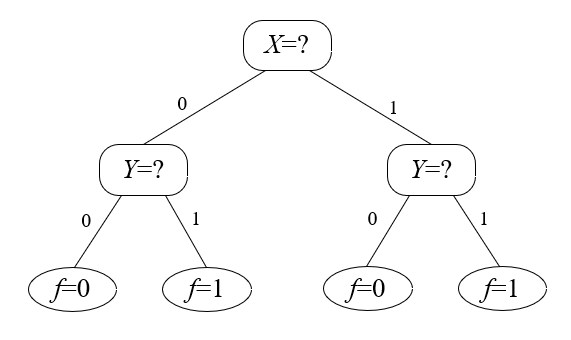
\includegraphics[scale=0.7]{p1-dt1.PNG}
	\end{figure}

	\noindent (2) 根结点的信息熵为
	\begin{align*}
		\text{Ent}(D)=-\sum\limits_{k=1}^2 p_k log_2 p_k
		=-(\frac{4}{10}log_2\frac{4}{10}+\frac{6}{10}log_2\frac{6}{10})
		=0.97095
	\end{align*}

	对属性$x_1$,将样本中$x_1$的取值从小到大排序,将$\frac{x_1^i+x_1^{i+1}}{2}$作为侯选划分点,得到
	\begin{align*}
		T_{x_1}=\{22.5,23.5,24.5,28.5,37.5,45.5,50,52,52.5\}
	\end{align*}
	依次计算
	\begin{align*}
		\text{Gain}(D,x_1,x_1^i)
		=\text{Ent}(D)-\sum\limits_{v=1}^2\frac{|D^v|}{|D|}\text{Ent}(D^v)
	\end{align*}
	得到
	\begin{align*}
		& \text{Gain}(D,x_1,22.5)=0.07898,\text{Gain}(D,x_1,23.5)=0.00740,\text{Gain}(D,x_1,24.5)=0.00580 \\
		& \text{Gain}(D,x_1,28.5)=0.04644,\text{Gain}(D,x_1,37.5)=0.12451,\text{Gain}(D,x_1,45.5)=0.01997 \\
		& \text{Gain}(D,x_1,50)=0.09128,\text{Gain}(D,x_1,52)=0.00740,\text{Gain}(D,x_1,52.5)=0.14448
	\end{align*}
	$x_1$信息增益为0.14448,对应划分点52.5。

	对属性$x2$,有
	\begin{align*}
		T_{x_2}=\{26,32.5,39,42,46,50,58.5,71,93.5\}
	\end{align*}
	\begin{align*}
		& \text{Gain}(D,x_1,26)=0.14448,\text{Gain}(D,x_1,32.5)=0.32193,\text{Gain}(D,x_1,39)=0.09128 \\
		& \text{Gain}(D,x_1,42)=0.019973,\text{Gain}(D,x_1,46)=0.12451,\text{Gain}(D,x_1,50)=0.04644 \\
		& \text{Gain}(D,x_1,58.5)=0.28129,\text{Gain}(D,x_1,71)=0.17095,\text{Gain}(D,x_1,93.5)=0.07898
	\end{align*}
	$x_2$信息增益为0.32193,对应划分点32.5。
	因此,以$x_2$为根节点划分属性。

	对于下一层的左结点,划分出的样本标记都为0,无需继续划分。
	对于右结点,可按照上述计算出
	$x_1$信息增益为0.31128,对应划分点37.5;
	$x_2$信息增益为0.20443,对应划分点58.5。
	因此,以$x_1$为该节点划分属性。

	对于下一层的左结点,划分出的样本标记都为1,无需继续划分。
	对于右结点,可按照上述计算出
	$x_1$信息增益为0.31128,对应划分点45.5和52.5;
	$x_2$信息增益为1,对应划分点58.5。
	因此,以$x_2$为该节点划分属性。

	对于下一层的左结点,划分出的样本标记都为0,无需继续划分。
	对于右结点,划分出的样本标记都为1,无需继续划分。

	决策树如下图所示:
	\begin{figure}[H]
		\centering
		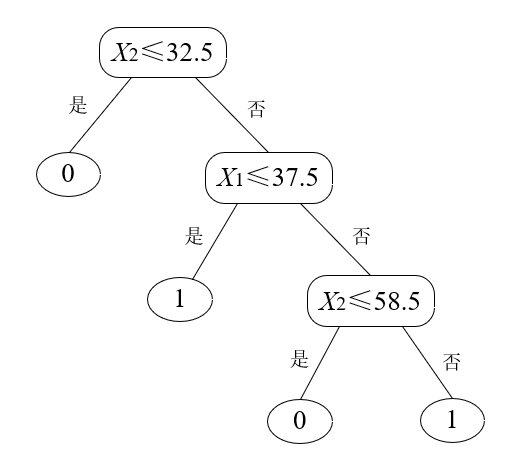
\includegraphics[scale=0.7]{p1-dt2.PNG}
	\end{figure}

	该决策树的分类误差为0。
	



	\newpage
	\section{[20pts] Neural Network}
	\noindent Consider the following neural network, consisting of two input units, a single hidden layer containing two units, and one output unit:
	
	\begin{figure}[htbp]
		\centering
		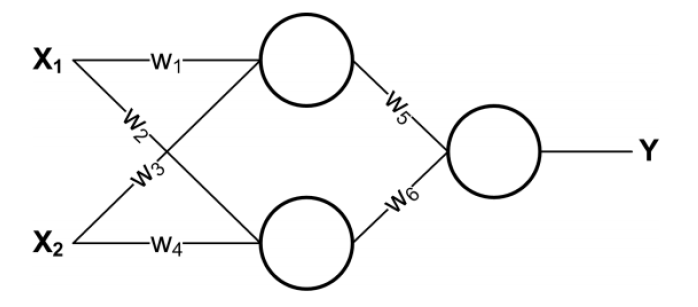
\includegraphics[scale=0.5]{p2-nn1.png}
	\end{figure}

	(1) [5pts] Assume that the network is using linear units: that is, for a given unit $U$, $A$ is the vector of activations of units that send their output to $U$ and $W$ is the weight vector corresponding to these outputs, then the output of the unit is $W^{\mathrm{T}}A$. Let the weight values $w_i$ be fixed, re-design the neural network to compute the same function without using any hidden units. Express the new weights in terms of the old weights.
	
	(2) [5pts] Is it always possible to express a neural network made up of only linear units without a hidden layer?
	
	(3) [10pts] Choose an activation function for each unit in the network which will cause this network to learn the same function that logistic regression would learn. Each unit should use a logistic, linear, or threshold activation function, with no constraints on the weights.
	\\
	
	\noindent 解:
	(1) 新的神经网络如下图所示:
	\begin{figure}[htbp]
		\centering
		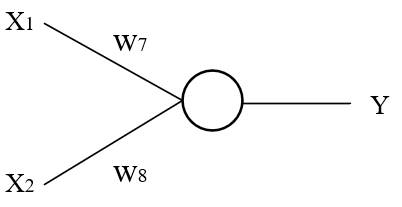
\includegraphics[scale=0.7]{p2-nn2.png}
	\end{figure}
	
	\noindent 其中$w_7=w_1w_5+w_2w_6$,$w_8=w_3w_5+w_4w_6$。

	\noindent (2) 
	总是能以没有隐藏层的形式表示一个仅由线性单元构成的神经网络。
	因为由线性单元构成的神经网络的输出总是能够用矩阵乘法表示,
	以题中的神经网络为例,输出可以表示为:
	\begin{align*}
		& Y=w_5(w_1x_1+w_3x_2)+w_6(w_2x_1+w_4x_2) \\
		& =(w_1w_5+w_2w_6)x_1+(w_3w_5+w_4w_6)x_2 \\
		& =\left[
			\begin{matrix}
				w_5 & w_6
			\end{matrix}
			\right] 
			\left[
			\begin{matrix}
				w_1 & w_3 \\
				w_2 & w_4
			\end{matrix}
			\right]
			\left[
			\begin{matrix}
				x_1 \\
				x_2
			\end{matrix}
			\right]
	\end{align*}
	因此,如果网络有$n$个输入,分别为$x_1,x_2,\dots ,x_n$,
	输出可以表示为:
	\begin{align*}
		Y=B_mB_{m-1}\dots B_1
		\left[
		\begin{matrix}
			x_1 & x_2 & \dots & x_n
		\end{matrix}
		\right]^{\mathrm{T}}
	\end{align*}
	其中$B_j$为每一层的权重构成的矩阵。
	那么,将各个输入$x_i$直接与输出层神经元相连,
	令其权重为$B_mB_{m-1}\dots B_1$乘积中第$i$列元素的值,
	即可得到符合题意的不含隐藏层的神经网络。

	\noindent (3) 
	令隐藏层上下两个神经元分别为$E$和$F$,输出层神经元为$G$。\\
	$E$的激活函数为$f_1(x)=x$,
	输出为$f_1(W_1^{\mathrm{T}}A)=w_1x_1+w_3x_2$,
	其中
	$$
		W_1=\left[
		\begin{matrix}
			w_1 \\
			w_3
		\end{matrix}	
		\right], 
		A=\left[
		\begin{matrix}
			x_1 \\
			x_2
		\end{matrix}	
		\right]
	$$
	$F$的激活函数为$f_2(x)=x$,
	输出为$f_2(W_2^{\mathrm{T}}A)=w_2x_1+w_4x_2$,
	其中
	$$
		W_1=\left[
		\begin{matrix}
			w_2 \\
			w_4
		\end{matrix}	
		\right]
	$$
	$G$的激活函数为$f_3(x)=(1+e^{-x})^{-1}$,
	输出为
	$$
	f_3(W_3^{\mathrm{T}}A_1)=(1+e^{-(w_1w_5+w_2w_6)x_1+(w_3w_5+w_4w_6)x_2})^{-1}
	$$
	其中
	$$
		W_3=\left[
		\begin{matrix}
			w_5 \\
			w_6
		\end{matrix}	
		\right], 
		A_1=\left[
		\begin{matrix}
			w_1x_1+w_3x_2 \\
			w_2x_1+w_4x_2
		\end{matrix}	
		\right]
		=\left[
		\begin{matrix}
			W_1^{\mathrm{T}} \\
			W_2^{\mathrm{T}}
		\end{matrix}	
		\right]A
	$$





	\newpage
	\section{[60 pts] Neural Network in Practice}
	
	\noindent In this task, you are asked to build a Convolutional Neural Networks (CNNs) from scratch and examine performance of the network you just build on \textbf{MNIST} dataset.
	Fortunately, there are some out-of-the-box deep learning tools that can help you get started very quickly. For this task, we would like to ask you to work with the \textbf{Pytorch} deep learning framework. Additionally, Pytorch comes with a built-in dataset class for MNIST digit classification task in the \textbf{torchvision} package, including a training set and a validation set. You may find a pytorch introduction at \href{https://pytorch.org/tutorials/beginner/blitz/cifar10_tutorial.html}{here}. Note that, you can use CPU or GPU for training at your choice.
	
	Please find the detailed requirements below.\\

	(1) [5 pts] You are encouraged to implement the code using \emph{Python3}, implementations in any other programming language will not be judged. Please name the source file (which contains the main function) as \emph{CNN\underline{\hspace{0.5em}}main.py}. Finally, your code needs to print the performance on the provided validation set once executed.
		    
	(2) [20 pts] Use any type of CNNs as you want and draw graphs to show your network architecture in the submitted report. You are encouraged to try more architectures.
		    
	(3) [25 pts] During training, you may want to try some different optimization algorithms, such as SGD, Adam. Also, you need to study the effect of learning rate and the number of epoch, on the performance (accuracy).
		    
	(4) [10 pts] Plot graphs (learning curves) to demonstrate the change of training loss as well as the validation loss during training.

	\noindent 
	解:(1)

	\noindent 
	(2)

	\noindent 
	(3)

	\noindent 
	(4)



\begin{thebibliography}{1}
%\bibitem{ref1} 周志华. 机器学习[M]. 清华大学出版社, 2016.
%\bibitem{ref2} 数据标准化/归一化\\\url{https://www.cnblogs.com/pejsidney/p/8031250.html}
\end{thebibliography}





\end{document}